\chapter{Contraction Hierarchies}\label{chapter:ch}

Eine Methode um in Graphen sehr schnell kürzeste Pfade zu berechen, sind Contraction Hierachies.
Die von \cite{geisberger2008contraction} vorgestellte Methode nutzt ein änliches Konzept zu der in \autoref{graphs:strassengraphen} Idee der Wichtigkeit auf und funktioniert deshalb für Straßengraphen sehr gut.
Die Grundidee der Suche eines kürzesten Pfades ist ein Bidirectionale Suche, welche jeweils nur wichtigere Knoten besucht.
Durch diese Enschränkung des Suchhraums kann, je nach dem Graphentyp, ein Speedup mehrerer Größenordnungen erreicht werden.

Wie zu sehen sein wird, lässicht sich die klassischen Methode zur Erstellung der benötigten Datenstrukturen nur bedingt auf Sichtbarkeitsgraphen anwenden.
Daher wird im follgenden zuerst unabhängig von der Erstellung argumentiert um später mehre Methoden hierfür vorzustellen.

Contraction Hierarchies bauen auf der Notation eines \emph{Levels} auf, jedem Knoten wird ein Level zugeorndet.
Diese kann als ein Grad der Wichtigkeit verstanden werden:
Je höher ein Level ist, desto wichtiger ist der Knoten im Allgemeinen für das Finden von kürzesten Pfaden.

\begin{definition}[Level]
    Sei $G = (V, E)$ ein Graph.
    Sei $L \subseteq \mathbb{N}$ mit $\abs{L} = \abs{V}$.
    Dann wird eine bijketive Funktion ${vtl} \coloneq V \to L$ \emph{vertex-to-level} Funktion genannt.
    Ihre Umkehrfunktion ${ltv}$ wird \emph{level-to-vertex} Funktion genannt.
\end{definition}

Die ein Level aus genau einem Knoten besteht, ist keine zwingen Notwendigkeit
So setzt \cite{vetter2009parallel} etwa mehrere Knoten auf einem Level, um das Preprocessing zu beschleunigen.
Die in dieser Arbeit verwende Einschränkung vereinfacht allerdings die Argumentation.

Bassierend auf dem Level kann der \emph{upward Graph} definiert werden.
Der Name des upward Graphen ergibt sich daher, dass die Suche in einem upward Graph auf das Level bezogen nur \emph{aufwärts} geht.
Formal ist dieser definiert als:

\begin{definition}[Upward Graph]
    Sei $G = (V, E)$ und ${vtl}$ eine \emph{vertex-to-level} Funktion dazu. Dann ist $G_u = (V, E_u)$ ein \emph{upward Graph} zu $G$ wenn gilt:
    \begin{enumerate}
        \item\label{ch:definition:legal_edges}
        $E_u$ enthält nur Kanten $(t, h, d)$ mit $t, h \in V$ und $d \in \mathbb{R}^+$, für die gillt, $d \geq {spd}_{G}((t, h))$ und es einen $(t, h)$ Pfad gibt, so dass $h$ das größte und $t$ das zweitgrößte Level auf diesem hat.

        \item\label{ch:definition:upward}
        $E_u$ enthält mindestens alle Kanten $(t, h, {spd}_{G}((t, h)))$ mit $t, h \in V$, für die gilt, dass $h$ das größte und $t$ das zweitgrößte Level auf allen kürzesten Wege auf $G$ von $t$ nach $h$ hat.
    \end{enumerate}
\end{definition}


Betrachten wir das ganze an dem bereits definierten Beispielgraph.
Sei ${vtl}$ definiert durch die Abbildung in \autoref{ch::fig::vtl_abbildung} definiert.
Durch Anwendung der Regel \ref{ch:definition:upward} ergibt sich der in \autoref{ch::fig::upward_graph} gezeigte upward Graph.
Es ist hierbei zu erwähnen, dass keine zusätzlichen Kanten nach \autoref{ch:definition:legal_edges} eingefügt wurden.

Der enstande Graph ist azyklisch, da er nur Kanten enthält, deren Kopf ein größeres Level als ihr Fuß hat.
Die Anzahl der in einer Breitensuche gefunden Knoten ist geringer, als im Ursprungsgraph.
Diese beiden Eingeschaften sorgen dafür, dass eine Suche in einem upward Graph kostengünstiger sei kann.
Die in einem upward Graph gefunden kürzesten Pfade bilden eine untere Grenze für kürzeste Pfade.

\begin{table}[ht]
    \centering
    \begin{tabular}{lllllllllllll}
        Vertex & a & b & c & d & e & f & g & h & i & j  & k & \\
        Level  & 8 & 7 & 3 & 6 & 2 & 5 & 1 & 4 & 0 & 10 & 9 &
    \end{tabular}
    \caption{${vtl}$ Beispielfunktion}
    \label{ch::fig::vtl_abbildung}
\end{table}


\begin{figure}[ht]
    \centering
    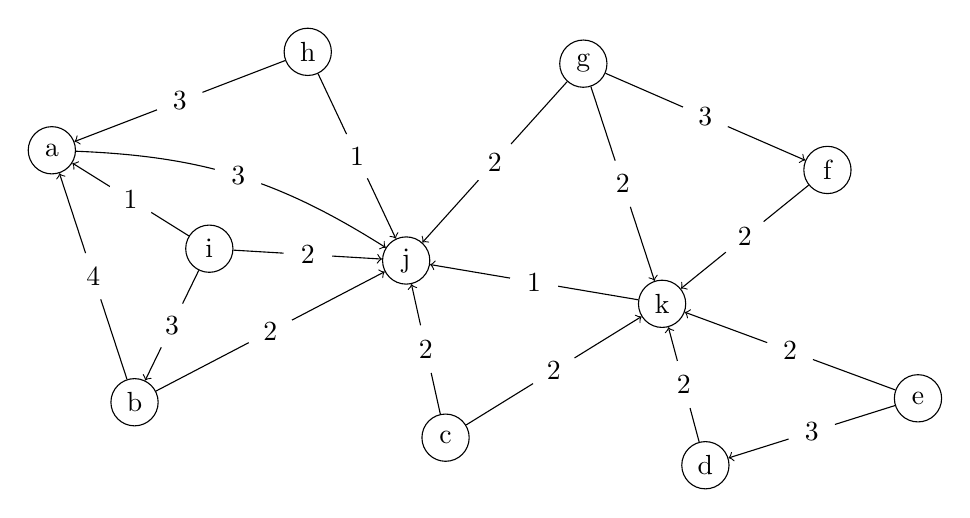
\begin{tikzpicture}
        % Nodes
        \node[circle, draw, minimum size=0.6cm, inner sep=0pt] at (0.5* 0.0, 0.5* 8.5)  (a)    {a};
        \node[circle, draw, minimum size=0.6cm, inner sep=0pt] at (0.5* 2.1, 0.5* 2.1)  (b)    {b};
        \node[circle, draw, minimum size=0.6cm, inner sep=0pt] at (0.5* 10.0, 0.5* 1.2)  (c)    {c};
        \node[circle, draw, minimum size=0.6cm, inner sep=0pt] at (0.5* 16.6, 0.5* 0.5)  (d)    {d};
        \node[circle, draw, minimum size=0.6cm, inner sep=0pt] at (0.5* 22.0, 0.5* 2.2)  (e)    {e};
        \node[circle, draw, minimum size=0.6cm, inner sep=0pt] at (0.5* 19.7, 0.5* 8.0)  (f)    {f};
        \node[circle, draw, minimum size=0.6cm, inner sep=0pt] at (0.5* 13.5, 0.5* 10.7)  (g)    {g};
        \node[circle, draw, minimum size=0.6cm, inner sep=0pt] at (0.5* 6.5, 0.5* 11.0)  (h)    {h};
        \node[circle, draw, minimum size=0.6cm, inner sep=0pt] at (0.5* 4.0, 0.5* 6.0)  (i)    {i};
        \node[circle, draw, minimum size=0.6cm, inner sep=0pt] at (0.5* 9.0, 0.5* 5.7)  (j)    {j};
        \node[circle, draw, minimum size=0.6cm, inner sep=0pt] at (0.5* 15.5, 0.5* 4.6)  (k)    {k};


        \draw[->]  (a) edge[bend left=15] node[circle, fill=white] {3} (j);

        \draw[->]  (b) edge node[circle, fill=white] {4} (a);
        \draw[->]  (b) edge node[circle, fill=white] {2} (j);

        \draw[->]  (c) edge node[circle, fill=white] {2} (j);
        \draw[->]  (c) edge node[circle, fill=white] {2} (k);

        \draw[->]  (d) edge node[circle, fill=white] {2} (k);

        \draw[->]  (e) edge node[circle, fill=white] {3} (d);
        \draw[->]  (e) edge node[circle, fill=white] {2} (k);

        \draw[->]  (f) edge node[circle, fill=white] {2} (k);

        \draw[->]  (g) edge node[circle, fill=white] {3} (f);
        \draw[->]  (g) edge node[circle, fill=white] {2} (j);
        \draw[->]  (g) edge node[circle, fill=white] {2} (k);

        \draw[->]  (h) edge node[circle, fill=white] {3} (a);
        \draw[->]  (h) edge node[circle, fill=white] {1} (j);

        \draw[->]  (i) edge node[circle, fill=white] {1} (a);
        \draw[->]  (i) edge node[circle, fill=white] {3} (b);
        \draw[->]  (i) edge node[circle, fill=white] {2} (j);


        \draw[->]  (k) edge node[circle, fill=white] {1} (j);
    \end{tikzpicture}
    \caption{Upward Graph des Beispielgraphs}
    \label{ch::fig::upward_graph}
\end{figure}

Die Suche eines kürzesten Pfades ist dann eine bidirectionale Suche, wobei die Suchen auf verschiedenen Graphen arbeiten.
Daher muss noch das Gegenstück das upward Graphens definiert werden, der \emph{downard Graph}.

\begin{definition}[Downward Graph]
    Sei $G = (V, E)$ und ${vtl} \coloneq V \to \mathbb{N}$ eine \emph{vertex-to-level} Funktion. Dann ist ein upward Graph des Umkehrgraphens $G^T$ ein \emph{downward Graph} zu $G$.
\end{definition}

Wenn ein Graph ungerichtet ist, dann ist er äuivalent zu seinem Umkehrgraphen und dann ist auch der Upward und Downward Graph äuivalent.
Daher entspricht \autoref{ch::fig::upward_graph} gleichzeitig auch dem Downward Graph des Beispielgraphens.

\section{Query}

Ein \emph{Contracted Graph} $C = (G_u, G_d)$ ist die Datenstruktur, mit deren Hilfe schnell kürzeste Wege gefunden werden können.
Sie besteht aus einem upwarward und downward Graph, wobei beide es eine ${vtl}$ Funktion geben muss, nach der Beide gültig sind.

Die Suche eines kürzesten Pfades von $a$ nach $e$ auf dem Beispielgraph gestaltet sich nun wie folgt:
Auf $G_u$ wird eine Dijkstra Suche von $a$ und auf $G_d$ eine Dijkstra Suche von $e$ durchgeführt.
Aus den von beiden besuchten Knoten wird derjenige ausgewählt, der die niedrigste Summe beider Distanzen hat.
\autoref{fig:ch:beispiel_suche} zeigt einen auf diese Weise gefunden Pfad auf dem Beispielgraph von $a$ nach $e$.
Es ist ersichtlich, dass die Level der Knoten auf dem Pfad zum Treffpunkt-Knoten $j$ ansteigen, bis schließlich der Knoten auf dem Pfad mit dem höchstem Level gefunden wird.
Die Kante $(a, j)$ ist hierbei ein Abkürzung, sie kürzt $i$ ab, was durch die gestrichelten Pfeile angedeuted wird.

\begin{figure}[ht]
    \centering
    \begin{tikzpicture}
        \node[circle, draw] at (0 * 1.5, -2 * 0.75)  (a)    {a};
        \node[circle, draw] at (1 * 1.5, -4 * 0.75)  (i)    {i};
        \node[circle, draw] at (2 * 1.5, -0 * 0.75)  (j)    {j};
        \node[circle, draw] at (3 * 1.5, -1 * 0.75)  (k)    {k};
        \node[circle, draw] at (4 * 1.5, -3 * 0.75)  (e)    {e};

        % draw axis
        \draw[->] (-1, -4 * 0.75) -- (-1, 0) node[above] {Level};

        \draw[->]  (a) -- (j);
        \draw[->]  (e) -- (k);
        \draw[->]  (k) -- (j);

        \draw[->, dotted]  (a) -- (i);
        \draw[->, dotted]  (i) -- (j);

    \end{tikzpicture}
    \caption{Beispiel einer Suche im Contrated Graph}
    \label{fig:ch:beispiel_suche}
\end{figure}

Algorithmus \ref{ch:query_simple} definiert den Aglorithmmus formal.
Wie bei einer Bidirectionalen Dijkstra Suche wird der Pfad, sofern dieser existiert, aus den Teilpgaden beider Suchen erstellt.
Diese haben die Form $(u, \dotsc, t)$ bzw. $(v, \dotsc, t)$.
Um einen gültigen Pfad zu erstellen, muss $t$ aus einem dieser Teilpfade entfernt werden und der Pfad des Downward Graphens umkegehrt werden.
Anschließend können beide Pfade verkettet werden und es ensteht ein Pfad auf $C$ der Form $(u, \dotsc, t, \dotsc, v)$.
Dieser Pfad muss aber kein Pfad auf $G$ sein, da er noch Abkürzungen enthalten kann.
In \autoref{ch:subsection:pfad_gewinnung} wird darauf eingegangen, wie diese entfernt werden können.

\begin{algorithm}[ht]
    \caption{Construction Hierachies Query}
    \begin{algorithmic}[1]
        \Require Upward-Graph $G_u = (V, E_u)$, Downward-Graph $G_d = (V, E_d)$, Startknoten $s \in V$, Zielknoten $t \in V$
        \Ensure Treffknoten $m \in V \cup \{ {none} \}$, ${dist}_u$, ${pre}_u$, ${dist}_d$, ${pre}_d$
        \State ${dist}_u$, ${pre}_u$ $\leftarrow$ Dijkstra$(G_u, s)$
        \State ${dist}_d$, ${pre}_d$ $\leftarrow$ Dijkstra$(G_d, t)$

        \State
        \State $m \leftarrow {none}$
        \State $d \leftarrow \infty$
        \State

        \ForAll {$v \in V$}
        \If {${dist}_u(v) + {dist}_d(v) < d$}
        \State $m \leftarrow v$
        \State $d \leftarrow {dist}_u(v) + {dist}_d(v)$
        \EndIf
        \EndFor

        \State
        \State \Return $m$, ${dist}_u$, ${pre}_u$, ${dist}_d$, ${pre}_d$
    \end{algorithmic}
    \label{ch:query_simple}
\end{algorithm}

Die Korrektheit des Algorithmus ist nicht sofort ersichtlich, da nicht alle Kanten optimal sind und nur ein Teil aller Knoten besucht wird.
Der Beweis hierfür betrachten hierbei betrachtet einen kürzesten Pfad auf $G$ und argumentiert, warum dieser gefunden wird:

\begin{beweis}\label{ch:proof:correct}
    Der Beweis der Korrektheit folgt in zwei Schritten.

    \begin{enumerate}
        \item
              ${spd}_G ((u, v)) = d$ mit $d \neq \infty$ $\Rightarrow$ ${spd}_C((u, v)) = d$.

              Sei ${sp}((u, v))$ der kürzeste Pfad auf $G$ der unter allen kürzesten Pfaden den Knoten $t$ mit dem höchstem Level enthält.
              Erstelle aus diesem Pfad $(u, \dotsc, v)$ zwei Pfade: $(u, \dotsc, t)$ und $(v, \dotsc, t)$.

              Gehe durch $(u, \dotsc, t)$ und entferne alle Knoten, die einen niedrigeren Level als ihr Voränger haben.
              Die Tupel benachbarten Knoten im neu enstanden Pfad sind nach der Definition des upward Graph Kanten von $G_u$, und zwar solche, die ein optimales Kantengewicht haben.
              Daher wird $t$ im upward Graph mit optimaler Distanz gefunden.

              Analog dazu wird im Pfad $(v, \dotsc, t)$ mit $G_d$ argumentiert.

              Da $t$ in beiden Suchen mit optimalen Gewicht gefunden wird und auf dem kürzesten Pfad liegt, ist auch die optimale Distanz des kürzesten Pfades gefunden

        \item
              ${spd}_G ((u, v)) = \infty$ $\Rightarrow$ ${spd}_C((u, v)) = \infty$.

              Angenommen, es würde ein Pfad $(u, \dotsc, v)$ in C gefunden werden.
              Sei $t$ wieder der Knoten mit den höchstem Level auf diesem Pfad.

              Erstelle aus $(u, \dotsc, v)$ zwei Pfade: $(u, \dotsc, t)$ und $(v, \dotsc, t)$.
              Die Tuple benachbarter Knoten entsprechen wieder Kanten im Upward. bzw. Downward Graph.
              \todo{Gegenbeweis sauber führen}
    \end{enumerate}

    Daher gilt, die Suche der kürzesten Pfad Distanz in $C$ ist äquivalent zu der in $G$
    \qed
\end{beweis}

\subsection{Erstellung des Pfades}\label{ch:subsection:pfad_gewinnung}
Der in $C$ gefundene Pfad kann bisher noch Abkürzungen enthalten.
Damit der Pfad auch auf $G$ gültig ist, müssen diese ersetzt werden.
Hierfür ist eine Funktion notwendig, welche diese ersetzt.

\begin{definition}[Abkürzungsfunktion]
    Sei $G = (V, E)$ ein Graph, und $C = (G_u, G_d)$ ein Contracted Graph von $G$.
    Betrachte die Abkürzungen $(u, v)$ aus $C$ als Pfade.
    $S \coloneq V \times V \to V \cup \{ {none} \}$ ist eine \emph{Abkürzungsfunktion} von $C$, wenn eine endliche, rekursive Anwenden von $S$ auf die Abkürzungen einen gültigen Pfad in $G$ erzeugt.
\end{definition}

Das rekursive Ersetzten kann durch den Algorithmus \ref{ch:alg:shortcut_replacement} verwirklicht werden.

\begin{algorithm}[ht]
    \caption{Shortcut replacement}
    \begin{algorithmic}[1]
        \Require Pfad $p$ mit Abkürzungen, Abkürzungungsfunktion $S \colon V \times V \to V \cup \{ {none} \}$
        \Ensure Pfad $p'$ ohne Shortcuts

        \If {$\text{len}(p) == 1$}
        \State \Return $p$
        \EndIf
        \State

        \State $p' \leftarrow ()$
        \State

        \While {$\text{len}(p) >= 2$}
        \State $w \leftarrow \text{pop}(p)$
        \State $u \leftarrow \text{pop}(p)$
        \State $v \leftarrow S((u, w))$
        \State

        \If {$v \neq none$}
        \State $\text{push}(p, u)$
        \State $\text{push}(p, v)$
        \State $\text{push}(p, w)$
        \Else
        \State $\text{push}(p, u)$
        \State $\text{push}(p', w)$
        \EndIf
        \EndWhile

        \State
        \State $p' \leftarrow \text{reversed}(p')$

        \State
        \State \Return $p'$
    \end{algorithmic}
    \label{ch:alg:shortcut_replacement}
\end{algorithm}

\section{Early stop}

Bisher werden beiden Suchen vollständig ausgeführt.
Die Anzahl der besuchten Knoten hierbei ist zwar kleiner als im zugrundeliegenden Graphen, jedoch ist es trotzdem wünschenswert, wenn die Suche frühzeitig gestoppt werden könnte.

Bei einer bidirectionalen Dijkstra Suche reicht es aus, die Suche zu stoppen, sobald die Summer der kleinsten Abstände der Vorwärtwarteschlange größer als der kleinste gefundene Abstand ist.
Dies ist hier nicht hinreichend, das die Suche auf im Upward bzw. Downward Graph keinen \emph{Ball} in $G$ bildet.
Anders ausgedrückt, es ist nicht garantiert, dass sich die Suchen an ihrer Front treffen:
Es ist möglich, dass die Suche im upward Graphen einen Knoten trifft, welcher selbst und alle seiner Nachfolger bereits expandiert worden sind.
Daher kann die Suche erst gestoppt werden, wenn die kleinste Distanz beider Warteschlangen größer oder gleich der des bisher besten Treffpunkt-Knotens ist.

Dies stopt die Suche zwar fühzeitig, die Anzahl der expandierten Knoten, nachdem der beste Treffpunkt-Knoten gefunden wurde ist jedoch immernoch hoch.
\todo{Funke fragen: Kann man hier noch verbessern? Ich habe die Mischung CH und ALT noch nicht verstanden}.

\section{Stall-on-demand}

Die im upward und downard Graphen gefunden Distanzen müssen nicht optimal sein.
Für das finden einen küzesten Pfades sind jedoch nur die Knoten interesannt, deren Distanz optimal ist.
Es ist möglich den Suchraum durch \emph{stall-on-demand} zu verkleinern.
\todo{Funke nochmal die Details. Mache ich das gerade richtig?}


% https://cstheory.stackexchange.com/questions/23767/why-is-label-pruning-possible-with-hub-labeling
Aus dieser Definition folgt, dass der kürzeste Pfad zwischen zwei Knoten in $G_u$ ist also mindestens genausolang ist wie in $G$.
Der Pfad darf aber auch länger sein.

\todo{Zeiche zwei Suchbäume, jeweils in G und Gu}

Für die Suche sind aber nur Knoten interesannt, die tatsächlich kürzesten Pfad Abstand haben.

Wie kann man diese Knoten nun leicht rausfiltern?
Beim expanded eines Knoten prüft man, für die Nachbarn der Gegenrichtung:


\section{Erstellung}

Die Erstellung des Contrated Graphens kann auf zwei Wegen geschehen: Durch Kontraktion und Brute-Forcing.
Inwiefern letzter eine sinnvolle Option ist wird \todo{Results} zu sehen sein.

\subsection{Kontraktion}

Der Name Contraction Hierachies leitet sich aus Konzept der Knoten Kontraktion (contraction) ab.
Diese funktioniert wie folgt:

\begin{definition}[Knoten Kontraktion]
    Sei $G = (V, E)$ ein Graph. Sei $v \in V$ der zu kontraktierende Knoten. Er wird kontraktiert indem:

    \begin{enumerate}
        \item\label{ch:contraction:when_shortcut}
        für jeden Vorgänger $u \in V$ und jeden Nachfolger $w \in V$ von $v$ einen Kante $(v, w, {spd}(u, w))$ in $E$ eingefügt wird, wenn $v$ auf dem einzigen kürzesten Pfad zwischen $u$ und $v$ liegt.

        \item
              alle Kanen von und zu $v$ entfernt werden.
    \end{enumerate}
\end{definition}

Nach der Kontraktion $v$ ist also isoliert.
Um die Abkürzungen zu erzeugen kann von jedem Voränger eine veränderte Dijkstra zu jedem Nachfolger gemacht werden.
Bei dieser Suche werden keine Kanten von und zu dem Knoten $v$ begangen.
Ist Länge eines auf diese Weise gefunden $u-w$ Pfades länger als der Pfad $(u, v, w)$, so wird keine Abkürzung eingefügt.

Diese Operation erhält für die verbleibenden Knoten die kürzesten Pfade.
Betrachten wir dies wieder am Beispielgraph.
Sei $i$ der zu kontraktierende Knoten, die Nachbarn sind $a$, $b$, $j$ und $h$.
Die kürzesten Pfade von $\{a, b\}$, $\{b, j\}$, $\{h, j\}$ und $\{a, h\}$ führend nicht durch $i$.
Der von $\{a, j\}$ jedoch doch, daher wird eine Kante eingefügt.
\autoref{graphs:fig:example_contraction} zeigt den Graphen nach der Kontraktion.

\begin{figure}[ht]
    \centering
    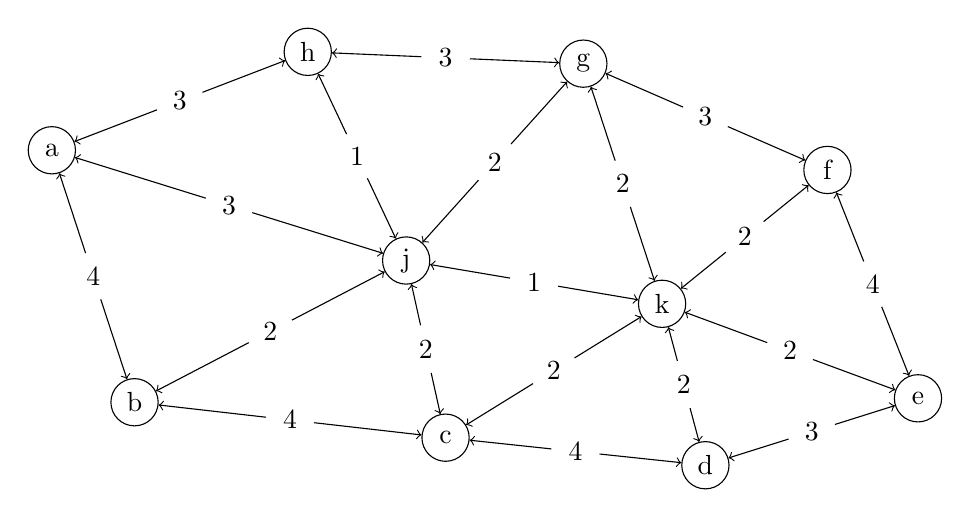
\begin{tikzpicture}
        % Nodes
        \node[circle, draw, minimum size=0.6cm, inner sep=0pt] at (0.5* 0.0, 0.5* 8.5)  (a)    {a};
        \node[circle, draw, minimum size=0.6cm, inner sep=0pt] at (0.5* 2.1, 0.5* 2.1)  (b)    {b};
        \node[circle, draw, minimum size=0.6cm, inner sep=0pt] at (0.5* 10.0, 0.5* 1.2)  (c)    {c};
        \node[circle, draw, minimum size=0.6cm, inner sep=0pt] at (0.5* 16.6, 0.5* 0.5)  (d)    {d};
        \node[circle, draw, minimum size=0.6cm, inner sep=0pt] at (0.5* 22.0, 0.5* 2.2)  (e)    {e};
        \node[circle, draw, minimum size=0.6cm, inner sep=0pt] at (0.5* 19.7, 0.5* 8.0)  (f)    {f};
        \node[circle, draw, minimum size=0.6cm, inner sep=0pt] at (0.5* 13.5, 0.5* 10.7)  (g)    {g};
        \node[circle, draw, minimum size=0.6cm, inner sep=0pt] at (0.5* 6.5, 0.5* 11.0)  (h)    {h};
        % \node[circle, draw, minimum size=0.6cm, inner sep=0pt] at (0.5* 4.0, 0.5* 6.0)  (i)    {i};
        \node[circle, draw, minimum size=0.6cm, inner sep=0pt] at (0.5* 9.0, 0.5* 5.7)  (j)    {j};
        \node[circle, draw, minimum size=0.6cm, inner sep=0pt] at (0.5* 15.5, 0.5* 4.6)  (k)    {k};


        \draw[<->]  (a) edge node[circle, fill=white] {4} (b);
        \draw[<->]  (a) edge node[circle, fill=white] {3} (h);
        \draw[<->]  (a) edge node[circle, fill=white] {3} (j);

        \draw[<->]  (b) edge node[circle, fill=white] {4} (c);
        \draw[<->]  (b) edge node[circle, fill=white] {2} (j);

        \draw[<->]  (c) edge node[circle, fill=white] {4} (d);
        \draw[<->]  (c) edge node[circle, fill=white] {2} (j);
        \draw[<->]  (c) edge node[circle, fill=white] {2} (k);

        \draw[<->]  (d) edge node[circle, fill=white] {3} (e);
        \draw[<->]  (d) edge node[circle, fill=white] {2} (k);

        \draw[<->]  (e) edge node[circle, fill=white] {4} (f);
        \draw[<->]  (e) edge node[circle, fill=white] {2} (k);

        \draw[<->]  (f) edge node[circle, fill=white] {3} (g);
        \draw[<->]  (f) edge node[circle, fill=white] {2} (k);

        \draw[<->]  (g) edge node[circle, fill=white] {3} (h);
        \draw[<->]  (g) edge node[circle, fill=white] {2} (j);
        \draw[<->]  (g) edge node[circle, fill=white] {2} (k);

        \draw[<->]  (h) edge node[circle, fill=white] {1} (j);

        \draw[<->]  (j) edge node[circle, fill=white] {1} (k);
    \end{tikzpicture}
    \caption{Beispielgraph}
    \label{graphs:fig:example_contraction}
\end{figure}

Um einen Contracted Graph zu erstellen, werden alle Knoten kontraktiert, wobei die Kanten, die in jedem Schritt entfernt werden, gesammelt werden.
Die Kanten, deren Kopf-Level größer ist, bilden die Kanten des Upward Graphens.
Die übrigen Kanten, also die deren Fußlevel größer ist, werden invertiert und bilden die Kanten des downard Graphens.
Diese Art der Erstellung erzugt zulässige Upward Graphen.
\todo{Beweis}

Häufig wird Kontraktionsbedingung abgeschwächt, es wird eine Kante eingefügt, wenn es \emph{wahrscheinlich} ist, dass auf dem einzig kürzesten Weg liegt.
Dazu kann eine normale Dijkstra Suche verwendet werden, es wird dann nur noch geprüft, ob der Knoten auf \emph{einem} kürzesten Pfad liegt.
Weiter kann die Anzahl der Hops der Suche begrenzt werden.
Dass hierbei mehr Kanten als notwendig eingefügt werden ist für die Korrektheit unproblematisch.
Das Einfügen unbenötigter Kanten kann jedoch einerseits den Speed negativ beinfluss, andererseits auch die Geschwindigkeit nachfolgenden Kontraktionen, da bei ihnen durch mehr Vorgänger mehr Dijkstra Suchen gemacht werden müssen.

Um die zu einem Contracted Graph dazugehörige Shortcut-Funktion zu erhalten, muss während der Kontraktion des Graphens eine Liste der Shortcuts erstellt werden.
Wird die im vorherigen Absatz erwähnte abgeschwächte Befingung verwenden, muss darauf geachtet werden, dass sich der kürzeste Shortcut zweier Knoten während der Kontraktion des Graphens mehrmals ändern kann.
Für die Shortcut-Funktion darf nur der als letzte gesetzte, beste Shortcut verwendet werden.

Die Reihenfolge, in der die Knoten kontraktiert wird (welcher der level-to-vertex Funktion ${ltv}$ entspricht), hat ebenfalls ein einen großen Einfluss auf den erzielten Speedup.

\subsubsection{Top-Down}

Bei der Top-Down Kontraktion ist die level-to-vertex Funktion ${ltv}$ vorgegeben.
Die Knoten werden in Reihenfolge ihres Levels kontrakiert, wobei mit dem niedrigsten Level begonnen wird.

\paragraph{Zufällig sortiert}
Die Knoten werden zufällig auf die Level verteilt. \todo{Funke fragen}

\paragraph{Sortiert nach Grad}
Die Knoten werden nach ihrem Grad sortiert, wobei die kleinsten Grade zuerst kontraktiert werden.
Die überlegung dahinter ist, dass Knoten mit vielen Nachbarn auch viele neue Kanten einfügen können, was vermieden werden soll.

\paragraph{Hitting Set}
Es wird ein Hitting Set über Pfade in $G$ erstellt.
Die Knoten welche am wenigsten Pfade treffen, werden zuerst kontraktiert.
Dies ist potentiell eine der besten Lösungen \todo{Oder? Kann man das beweisen?}.

\subsubsection{Bottom-Up}

Bei der Bottom-Up contraction wird die vertex-to-level Funktion ${vtl}$ währen der Kontraktion erstellt.
Dafür wird mit einer Heuristik der jeweils nächst \emph{unwichtigste} Knoten ausgewählt, kontraktiert und dem nächstem Level zugewiesen.
Ein unwichtiger Knoten hat hierbei einen niedrigen Heuristik-Wert.
Die in der Praxis am meist-verwendeten Heurisiken beinhalten die \emph{Kanten-Differenz}.
Sie gibt an wie sich die Anzahl der Kanten im gesammten Graph durch die Kontraktion verändert.
Sie wird durch die Anzahl der neu hinzugefügten Kanten subtrahiert durch die Anzahl der entfernten Kanten gebildet.
Die Kontraktion eines Knoten kann dabei die Heurisitk-Werte anderer Knoten verändern.
Damit jedes mal der Knoten mit der niedrigsten Heuristik ausgewählt wird, müssen nach jeder Kontraktion alle Heuristik-Werte neuberechnet werden.
Dies ist im Allgemeinen jedoch zu teuer ist, weshalb in der Praxis sich zwei Methoden als effektiv gezeigt haben:

Beim \emph{Lazy poping} besteht die Annahme, dass ein Knoten nur wichtiger werden kann.
Aus der Warteschlange wird ein Knoten entnommen und geprüft, ob sein Heuristik-Wert noch gleich ist.
Wenn er noch gleich ist, wird er kontraktiert, wenn nicht wird er zurück die Warteschlange gepusht.
Dies wird wiederholt, bis schließlich ein Knoten gefunden wird.

Beim \emph{Neighbor update} werden nach der Kontraktion eines Knoten die Heuristik Werte der Nachbarn geupdated.
Es lässt sich zeigen, dass sich die Kanten-Differenz von Nachbarn zweiter Ordnung nur in Ausnahmfällen ändert. \todo{cite}
Dies hat den Vorteil, dass dies für alle Nachbarn parallisiert passieren kann.

\subsubsection{Ideen}

Die bisher erwähnten Methoden eignen sich nur bedingt für Graphen mit großem durchscnittlichen Knotengrad.
Dieser wirkt sich auf die Erstellungzeit der Kanten-Differenz, da für jedes Paar aus Vorgänger und Nachfolger geprüft werden muss, ob bereits eine Kante zwischen ihnen exisitert.
Auch wenn dies durch eine passende Datenstruktur sehr effizient geschehen kann, kann dies sehr teuer sein:
Angenommen ein Knoten hat einen Grad von \num{10000}, dann müssen \num{100000000} viele Paare geprüft werden.
Bei einer angenommen Suchzeit von \num{10}\unit{\ns} pro Paar entspricht dies einer Sekunde.


Daher gibt es zwei Baustellen, die beschleunigt werden müssen:
Die Heuristik und die Kontraktion.

\paragraph{Kontraktion}
Anstatt einer teuren Suche kann auch eine Heuristik verwendet werden, welche eine obere Schranke angibt.
Dies ist insofern auch nicht abwägig, da die abgeschwächte Dijkstra Suche selbst nur eine obere Schranke angibt.
Eine Abkürzung wird dann eingefügt, wenn ihre Länge kleiner gleich einer oberen Schranke ist.
Falls es günstiger ist untere Schranken zu ermitteln, kann auch zuerst geprüft werden, ob die Länge gleich einer unteren Schranke ist, dann muss ebenfalls eine Abkürzung eingefügt werden.

\subparagraph{Triviale Heurisik}
Eine mögliche Idee ist, jede mögliche Abkürzung einzufügen, also die obere Schranke $\infty$ zu wählen.
Unter der Annahme, dass bei einem sehr hohem Kantengrad fast alle Vorgänger bereits Kanten zu fast allen Nachfolgern haben, ist der Anteil der unötig eingefügenten Kanten zu den notwendig eingefügten Kanten vielleicht vertertbar.
Die Berechnung der Kanten-Differenz und der Kontraktion sind dabei ebenfalls gleich, was beim Lazy-Popping praktisch ist, da dann die neuberechnung der Heuristik ebenfalls die neuen Kanten liefert.

\subparagraph{Vereinfacher Graph}
Gibt es einen vereinfachten Graphen $G'$, der obere Schranken zu $G$ für alle Knotenpaare liefert, dann kann auf diesem gesucht werden.
Insbesondere kann eine auf $G'$ angwendet Speedup-Technik verwendet werden, wie etwe Contraction Hierarchies oder Hub Labels.

\subparagraph{Dreickunsgleichung}
Ähnlich zu ALT\cite{goldberg2005computing} kann eine Menge Landmarks berechnet werden, welche mittels der Dreiecksungleichung eine obere Schranke angeben können.
Ein Landmark ist hierbei ein Knoten, für den die Distanz zu und von allen Knoten bekannt ist.
Hierbei gilt für ein Landmark $l \in V$, dass für alle $u, v \in V$ mittels ${spd}((u, l)) + {spd}((l, u))$ eine obere Schranke bestimmt werden kann.
Liegt $l$ dabei auf einem kürzesten Pfad von $u$ nach $v$, so entspricht der Wert sogar genau dem der kürzesten Pfad Distanz.
Damit durch ein möglichst kleine Menge an Landmarks eine möglichst große Menge an Pfaden abgeckt wird, müssen diese ein Hitting Setüber eine möglichst große Menge an Pfaden bilden.

Die Methoden der Dreicksungleichung und des Vereinfachten Graphens können auch kombiniert werden, wobei die jeweils kleinere obere Schranke ausgewählt wird.
Die Hoffnung hierbei ist, dass der Vereinfachte Graph Kanten mit einem niedrigen Hop-Abstand gut abschätzen kann, die Dreiecksungleichung gut Pfade mit einem hohen Hop Abstand, da die Wahrscheinlichkeit dass ein Landmark auf oder nahe einem kürzesten Pfad ist dann steigt.

\paragraph{Propabalistische Heuristik}
Wie bereits erwähnt wird bei großen Kantengraden die Berechnung der Kanten-Differenz sehr teuer.
Eine Idee diese Kosten anzufangen, ist es die Kanten-Differenz heuristisch anzuhnähern.
Dafür wird eine Teilmenge aller Vorgänger, Nachfolgerpaare gebildet für die die Kanten-Differenz gebildet wird.
Dieses Ergebnis wird dann auf die tatsächliche Menge an Paaren skaliert.
Dies kann nicht ohne weiteres mit Lazy Popping zusammen verwendet werden, da sich das die Ergebnisse bei zwei aufraufen hinterinander unterscheiden kann.
Dies kann dazu führen, dass unötigt oft Lazy gepoppt wird.

\paragraph{Layz Popping}
Bei normalen Lazy Popping wird ein Knoten zurückgepusht, wenn er nicht mehr den gleichen Heuristik-Wert wie zuvor hat.
Dies könnte angepasst werden, so dass ein gewisse Abweichung, entweder absolut oder relativ, zulässig ist.

\paragraph{Neighbor update}
Anstatt jeden Nachbar sofor upzudaten kann für jeden Nachbarn mitgezählt werden, wie oft ein Nachbar kontraktiert wurde.
Erst wenn dies einen gewissen Schwellwert überschritten hat, wird der Knoten geupdated.

\paragraph{Neubrechnung alle $n$ kontraktionen}
Die Heuristik-Werte werden all $n$ Kontraktionen für alle Knoten neuberechnet.

\section{Brute force}

Die in der Defintion des upward Graphens genannten Kanten könnne auch berechnet werden, indem für jede Graphe eine angepasste Dijkstra Suche durchgeführt wird.
Dafür wird während der Dijstra Suche notiert, was das größte Level auf dem Weg von der Wurzel bis zu dem Knoten ist.
Ein Knoten ist der Kopf eine CH Kante, für die gilt, dass das größte Level auf dem Weg zur Wurzel zu ihr sie selber hat und der größte Level des Vorgängers der der Wurzel ist.
Das Gewicht der Kante kann Dijkstra entommen werden.

Während es für Straßengraphen vermutlich deutlich teuer ist, kann es für ander Graphenklassen durchaus Sinn machen, wenn andere Methoden zur Erstellung eines Contracted Graphen noch teuerer sind.
Die Berechung ist \emph{embarrassingly parallel}, da jeder Knoten für sich selbst Berechnet werden kann, wobei das Erstellen der Abkürzungen, sofern benötigt, synchronisert werden sollte, um den Speichbedarf zu verkleinern.

\todo{Ich habe die Vermutung, dass theoretisch die Laufzeit pro Knoten für Bruteforce immer größer gleich all-in ist}

\subsection{Alogrithmus im Detail}

Betrachten wir wieder eine Suche vom Knoten $a$ im Beispielgraphen.
Ihr Suchbaum ist \autoref{ch:fig:brute_force_suchbaum} gezeigt.
Die Höhe der Knoten entspricht hierbei dem Zeitpunkt der Expansion, die linke Zahl steht für das dem Knoten zugewiesene Level, die rechte für das höchste Level auf dem Weg zzur Wurzel.
Die Definition des upward Graphens besagt, dass genau dann eine Kante $(u, v)$ eingefügt werden muss, wenn ${vtl}(v) > {vtl}(v)$ und es auf allen kürzesten Pfaden zwischen $v$ den höchsten und $u$ den zweithöchsten Level hat.
Für die Berechnung schwächen wir dies ab, und fügen eine Kante ein, wenn es einen kürzesten Pfad gibt, der dies erfüllt.
Hierfür tracken wir den höchsten Level, welcher auf dem Weg von der Wurzel zum Knoten bisher gesehen wurde.
Der erste Knoten auf dem jedem Weg von der Wurzel zum Blatt, für den gilt, dass er selbst das größte Level hat, bildet den Kopf einer Kante im upward Graph.


Die Suche muss dabei nicht bis zum Ende durchgeführt werden.
Es reicht so lange zu suchen, bis es keine Knoten mehr gibt, die noch nicht expandiert wurden und für die es auf dem Weg zur Wurzel nicht mindestens eine solche Kante gibt.
Hierfür wird eine Menge an \emph{lebendigen} Knoten benutzt.
Zu beginn ist nur der Startknoten lebendig, die Lebendigkeit wird jeweils an die Kinder vererbt.
Ein Knoten stirbt, nachdem er expandiert wurde oder wenn er den Kopf einer Kante bildet.
Gibt es keine lebendigen Knoten mehr, so kann die Suche abgebrochen werden.
In dem verwendeten Beispiel wäre dies etwa nach der Expansion von $b$ der Fall.


% \begin{algorithm}[ht]
%     \caption{Contracted Graph Brute Force Suchalgorithmus}
%     \begin{algorithmic}[1]
%         \Require Graph $G = (V, E)$, vertex-to-level Funktion ${vtl}$, Startknoten $s \in V$, Zielknoten $t \in V$
%         \Ensure $E_s$
%         \State // Initialisiere Distanz- und Vorgänger-Funktion
%         \ForAll{$v \in V$}
%         \State ${dist}(v) \leftarrow \infty$
%         \State ${pre}(v) \leftarrow {none}$
%         \EndFor
% 
% 
%         \State
%         \State // Initialisiere Vorrangwarteschlange
%         \State ${dist}(s) \leftarrow 0$
%         \State $Q\leftarrow \{ s \}$
% 
% 
%         \State
%         \State // Initialisiere max\_level\_path
%         \State ${mlp}(s) \leftarrow {vtl}(s)$
%         \State $E_s \leftarrow \{ \}$
%         \State ${alive} \leftarrow \{ s \}$
% 
%         \State
%         \While{$Q \neq \emptyset \land {alive} \neq \emptyset$}
%         \State $u \leftarrow{extract\_min}(Q)$\label{graphs:dijkstra:pop}
% 
%         \State
%         \State // Beende frühzeitig wenn Zielknoten gefunden wurde
%         \If {$u \neq s \land {mlp}(u) = {vtl}(u)$}
%         \State $E_s \leftarrow E_s \cup \{ (s, u, {dist}(u)) \}$
%         \State ${alive} \leftarrow {alive} \setminus \{ s \}$
%         \EndIf
% 
%         \State
%         \State // Aktualisiere Nachbarn
%         \ForAll{$(u, v, w) \in E$}
%         \If {${dist}(u) + w < {dist}(v)$}
%         \State ${dist}(v) \leftarrow {dist}(u) + w$
%         \State ${pre}(u) \leftarrow v$
%         \State $Q = Q \cup \{ v \}$
%         \State
%         \State // setze max\_level\_path
%         \State ${mlp}(v) \leftarrow \max({mlp}(v), {vtl}(v))$
%         \If {$u \in {alive}$}
%         \State ${alive} \leftarrow {alive} \cup \{ s \}$
%         \EndIf
%         \EndIf
%         \EndFor
% 
% 
%         \State ${alive} \leftarrow {alive} \setminus \{ s \}$
% 
%         \EndWhile
% 
%         \State
%         \State \Return $E_s$
%     \end{algorithmic}
% \end{algorithm}

\begin{figure}[ht]
    \centering
    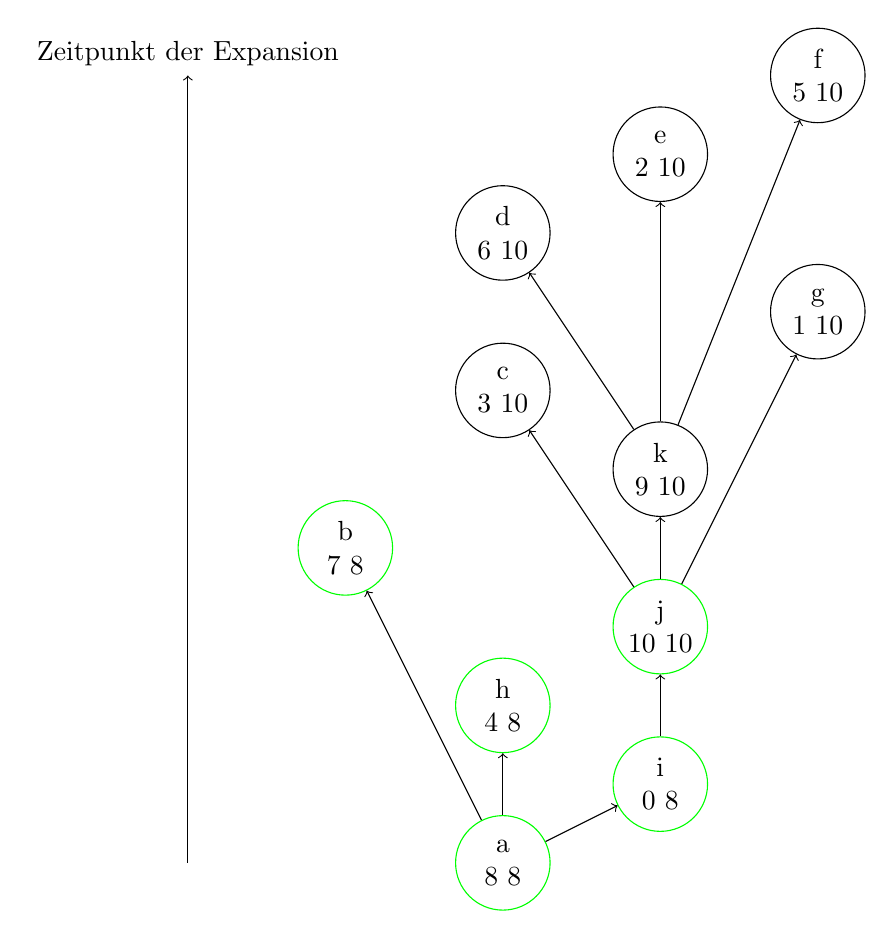
\begin{tikzpicture}
        % Nodes
        % a & b & c & d & e & f & g & h & i & j & k & 
        % 8 & 7 & 3 & 6 & 2 & 5 & 1 & 4 & 0 & 10 & 9 & 

        \node[circle, draw=green, minimum size=1.2cm, inner sep=0pt , align=center] at (2* 1, 0)  (a)    {a\\8 8};
        \node[circle, draw=green, minimum size=1.2cm, inner sep=0pt , align=center] at (2* 0, 4)  (b)    {b\\7 8};
        \node[circle, draw, minimum size=1.2cm, inner sep=0pt , align=center] at (2* 1, 6)  (c)    {c\\3 10};
        \node[circle, draw, minimum size=1.2cm, inner sep=0pt , align=center] at (2* 1, 8)  (d)    {d\\6 10};
        \node[circle, draw, minimum size=1.2cm, inner sep=0pt , align=center] at (2* 2, 9)  (e)    {e\\2 10};
        \node[circle, draw, minimum size=1.2cm, inner sep=0pt , align=center] at (2* 3, 10)  (f)    {f\\5 10};
        \node[circle, draw, minimum size=1.2cm, inner sep=0pt , align=center] at (2* 3, 7)  (g)    {g\\1 10};
        \node[circle, draw=green, minimum size=1.2cm, inner sep=0pt , align=center] at (2* 1, 2)  (h)    {h\\4 8};
        \node[circle, draw=green, minimum size=1.2cm, inner sep=0pt , align=center] at (2* 2, 1)  (i)    {i\\0 8};
        \node[circle, draw=green, minimum size=1.2cm, inner sep=0pt , align=center] at (2* 2, 3)  (j)    {j\\10 10};
        \node[circle, draw, minimum size=1.2cm, inner sep=0pt , align=center] at (2* 2, 5)  (k)    {k\\9 10};


        \draw[->]  (a) edge (b);
        \draw[->]  (a) edge (h);
        \draw[->]  (a) edge (i);
        \draw[->]  (j) edge (c);
        \draw[->]  (i) edge (j);
        \draw[->]  (k) edge (d);
        \draw[->]  (j) edge (k);
        \draw[->]  (k) edge (e);
        \draw[->]  (k) edge (f);
        \draw[->]  (j) edge (g);

        \draw[->] (-2, 0) -- (-2, 10) node[above] {Zeitpunkt der Expansion};

    \end{tikzpicture}
    \caption{Brute-Force Suche}
    \label{ch:fig:brute_force_suchbaum}
\end{figure}

\subsection{Abkürzung Problem}

Es liegt nahe als abgekürzten Knoten den Knoten mit dem dritthöchsten Level auszuwählen und sich darauf zu verlassen, dass die Suche von diesem Knoten aus die nächsen Abkürzung findet, und so weiter.
Dies wäre praktisch, da dann jeder Shortcut nur einmal erstellt werden müsste.
Zwei Gründe können jedoch dagegen sprechen:
Wird als Graph eine Datenstruktur verwendet, welche die Nachbarn nicht in einer definierten Ordnung ausgibt (etwa ein Hashset), können zwei Suchen von bzw. zu einem Knoten zwei Unterschiedliche kürzeste Pfad Bäume bilden.
Eine nicht stabile Prioritätswarteschlange kann ebenfalls den gleichen Effekt herbeiführen.

\autoref{ch:fig:problem_shortcut} zeigt eine Situation, in der so ein Problem auftreten kann.
Für den Knoten $a$ wird die Kante $(a, e)$ mit dem abekürztem Knoten $d$ gefunden.
Wir verlassen uns darauf, dass die Suche von $d$ aus die Abkürzung $(d, a)$ mit dem Knotem $b$ findet.

Die Lösung hierfür ist, dass die Abkürzungen, welche benötigt werden, um die ursprüngliche Abkürzung vollständiz zu entpacken, ebenfalls erstellt werden.
Diese werden aber mit einer hohen Wahrscheinlichkeit von den Bruteforcing der jeweils abgekürzten Knoten endeckt.
Der Speichermehrbedarf hierbei kann ein Problem für die Umsetzbarkeit des Algorithmus werden, weshalb ein Mechanismus verwendet werden sollte, welcher die mehrfache Speicherung verhindet, etwa eine HashMap.
Dies führt allerdings zu einem Performance-Hit, da dies synchroniesert werden muss.
Für denn Fall, dass nur die kürzesten Pfad Abstände Interesannt sind, kann und sollte hierauf verzichtet werden.

\begin{figure}[ht]
    \centering

    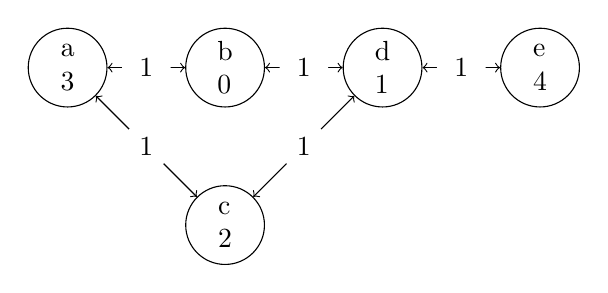
\begin{tikzpicture}
        % Nodes
        \node[circle, draw, minimum size=1cm, inner sep=0pt, align=left] at (2*0, 2*0)  (a)    {a\\3};
        \node[circle, draw, minimum size=1cm, inner sep=0pt, align=left] at (2*1, 2*0)  (b)    {b\\0};
        \node[circle, draw, minimum size=1cm, inner sep=0pt, align=left] at (2*1, 2*-1)  (c)    {c\\2};
        \node[circle, draw, minimum size=1cm, inner sep=0pt, align=left] at (2*2, 2*0)  (d)    {d\\1};
        \node[circle, draw, minimum size=1cm, inner sep=0pt, align=left] at (2*3, 2*0)  (e)    {e\\4};


        \draw[<->]  (a) edge node[circle, fill=white] {1} (b);
        \draw[<->]  (b) edge node[circle, fill=white] {1} (d);
        \draw[<->]  (d) edge node[circle, fill=white] {1} (e);


        \draw[<->]  (a) edge node[circle, fill=white] {1} (c);
        \draw[<->]  (c) edge node[circle, fill=white] {1} (d);
    \end{tikzpicture}
    \caption{Problem beim Shortcut erstellen}
    \label{ch:fig:problem_shortcut}
\end{figure}